\documentclass[12pt]{letter}
\usepackage{amsmath,amsfonts,amsthm,amstext,amssymb,graphicx, multicol,fancyhdr,lastpage,fullpage,framed,fancybox,enumerate,tikz,color,mathrsfs, polynom}
\usepackage[margin=0.6in,headsep=3pt, headheight=15pt]{geometry}

% ----------------------------------------------------------
% Custom Definitions, Commands, Environments, etc.

% Sets of numbers
\def\R{\mathbb{R}} % The reals
\def\N{\mathbb{N}} % The naturals
\def\Z{\mathbb{Z}} % The integers
\def\Q{\mathbb{Q}} % The rationals

% Blank space
\newcommand{\blank}[1]{\underline{\hspace{#1}}} % Blank space

% Change font colors
\newcommand{\cyan}[1]{{\color{cyan}{#1}}} % Changes font to cyan
\newcommand{\red}[1]{{\color{red}{#1}}} % Changes font to red
\newcommand{\magenta}[1]{{\color{magenta}{#1}}} % Changes font to magenta
\newcommand{\orange}[1]{{\color{orange}{#1}}} % Changes font to orange
\newcommand{\yellow}[1]{{\color{yellow}{#1}}} % Changes font to yellow
\newcommand{\violet}[1]{{\color{violet}{#1}}} % Changes font to violet
\newcommand{\green}[1]{{\color{green}{#1}}} % Changes font to green
\newcommand{\blue}[1]{{\color{blue}{#1}}} % Changes font to blue
\newcommand{\white}[1]{{\color{white}{#1}}} % Changes font to white

% Fitted inclusion symbols
\newcommand{\fp}[1]{\left({#1}\right)} % Fitted parentheses around content
\newcommand{\fb}[1]{\left[{#1}\right]} % Fitted brackets
\newcommand{\set}[1]{\left\{{#1}\right\}} % Fitted braces (useful for sets)
\newcommand{\av}[1]{\left|{#1}\right|} % Fitted absolute value bars

% Augmented Matrix Environment
\newenvironment{amatrix}[1]{%
	\left[\begin{array}{@{}*{#1}{c}|c@{}}
	}{%
	\end{array}\right]
}

% Miscellaneous
\def\then{\Rightarrow}
\def\to{\rightarrow}
\def\d{^{\circ}}
\newcommand{\?}{\stackrel{?}{=}}



% Coordinate Plane (Four-Quadrant)
\def\coordplane {
	\begin{tikzpicture}		\draw[step=0.25cm,black,very thin,opacity=0.25] (-2.5cm, -2.5cm) grid (2.5cm, 2.5cm);
	\draw[<->,thick,black] (-2.5cm, 0) -- (2.5cm, 0) node[anchor=north west,pos=0.94,font=\scriptsize]{$x$};
	\draw[<->,thick,black] (0,-2.5cm) -- (0, 2.5cm) node[anchor=south east,font=\scriptsize,pos=0.94]{$y$};
	\end{tikzpicture}
}

% Coordinate Plane (One-Quadrant)
\def\onequad {
	\begin{tikzpicture}
	\draw[step=0.25cm, black, very thin, opacity=0.25] (0,0) grid (7.5cm,5cm);
	\draw[->, thick, black] (0,0) -- (7.5cm, 0) node[anchor=north west,font=\scriptsize,pos=0.94]{$x$};
	\draw[->, black, thick] (0,0) -- (0,5cm) node[anchor=south east,font=\scriptsize,pos=0.94]{$y$};
	\end{tikzpicture}
}

% Counters
\newcounter{exercise}

% Exercise environment (auto-numbered)
\newenvironment{exercise}[1][]{\begin{framed}\refstepcounter{exercise}\textbf{Exercise~\theexercise:} #1}{\end{framed}}

% Book exercise environment
\newenvironment{bex}[2][] {
	\begin{framed}
		\textbf{Book Exercise {#2}}#1
	\end{framed}
}
% ----------------------------------------------------------

% ----------------------------------------------------------
% Header and Footer Information
% \pagestyle{fancy}
% \fancyhf{}
% \renewcommand{\headrulewidth}{0pt}
% \rhead{Name: \blank{2in}}
% \lhead{@}
% \rfoot{Page \thepage \, of \,\pageref{LastPage}}
% ----------------------------------------------------------
\author{Jacob Ayers}

\begin{document}
	\textbf{Assignment 7 Key \\ MAT 130}
	\begin{bex}{3.5.10}
		{
			
		}
	\end{bex} \vspace{-8pt}
	
	% My answer here
	(a) 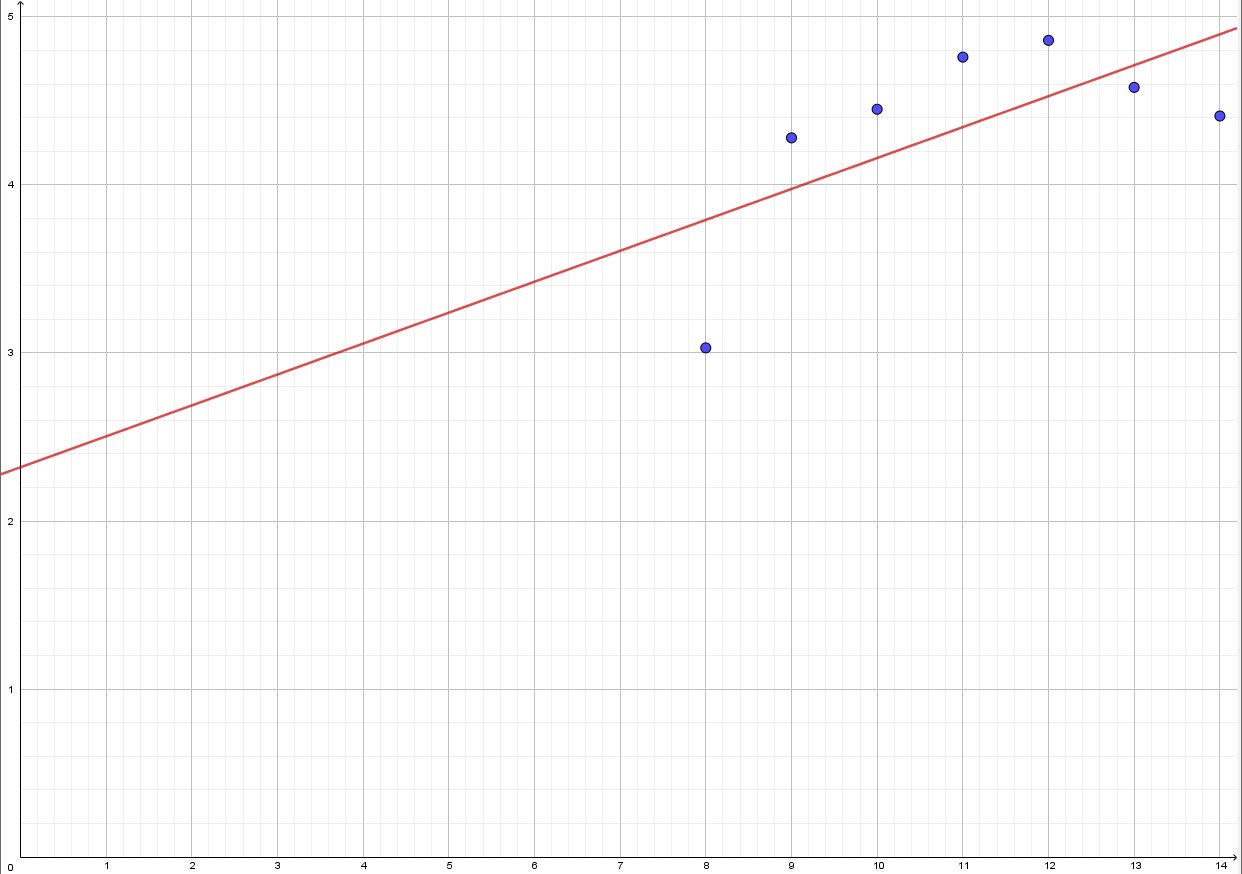
\includegraphics[width=3in]{3510a.png}
	
	(b) This model is not a very good fit for the data. Since the revenues start out rising, appear to achieve a maximum, then begin to decrease, a quadratic model would likely be a better fit.
	
	% \vspace{}
	\vfill % \newpage
	
	\begin{bex}{3.5.14}
		{
			
		}
	\end{bex} \vspace{-8pt}
	
	% My answer here
	Lines and equations will vary. My instinct was a line passing through the points $(0, 2)$ and $(5, 4)$. The slope of this line is $\dfrac25$ and its $y$-intercept is $2$, so my equation was $y = 0.4x + 2$. If your slope is close to $0.4$ (certainly should be larger than 0 and smaller than 0.6) and your $y$-intercept is close to $2$ (certainly should be between 1.75 and 2.25), then your answer would be acceptable.
	
	% \vspace{}
	\vfill % \newpage
	
	\begin{bex}{3.5.18}
		{
			
		}
	\end{bex} \vspace{-8pt}
	
	% My answer here
	(a) Using a TI-84 Plus \\ 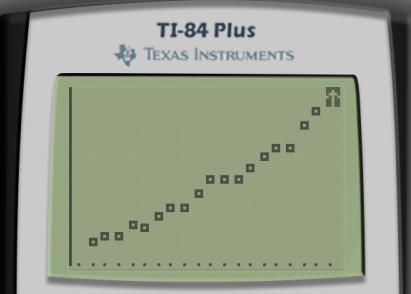
\includegraphics[width=2in]{3518a.png}
	
	(b) A TI-84 Plus gives the following equation: $S = 44.97832817t + 192.50258$.
	
	\vfill \newpage
	
	(c) Using a TI-84 Plus: \\ 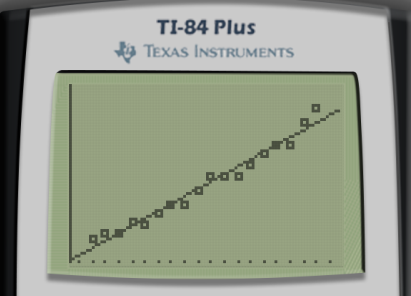
\includegraphics[width=2in]{3518c.png} \\
	This appears to be a good fit.
	
	(d) In 2021, $t = 31$. We need to find $S$ when $t = 31$. \\
	$S = 44.97832817(31) + 192.50258 = 1586.830753$
	
	(e) The slope tells us that the gross ticket sales for Broadway shows increase by about $45$ million dollars per year.
	
	% \vspace{}
	\vfill % \newpage
	
	\begin{bex}{3.5.40}
		{
			
		}
	\end{bex} \vspace{-8pt}
	
	% My answer here
	$V = kl^3$
	
	% \vspace{}
	\vfill % \newpage
	
	\begin{bex}{3.5.42}
		{
			
		}
	\end{bex} \vspace{-8pt}
	
	% My answer here
	$h = \dfrac{k}{\sqrt{s}}$
	
	% \vspace{}
	\vfill % \newpage
	
	\begin{bex}{3.5.44}
		{
			
		}
	\end{bex} \vspace{-8pt}
	
	% My answer here
	$z = kx^2y^3$
	
	% \vspace{}
	\vfill % \newpage
	
	\begin{bex}{3.5.46}
		{
			
		}
	\end{bex} \vspace{-8pt}
	
	% My answer here
	$P = \dfrac{k}{V}$
	
	% \vspace{}
	\vfill % \newpage
	
	\begin{bex}{3.5.54}
		{
			
		}
	\end{bex} \vspace{-8pt}
	
	% My answer here
	The model is of the form $A = kr^2$. We know that $A = 9\pi$ when $r = 3$. We can use this information to find $k$: \begin{flalign*}
	9\pi  &= k(3)^2 & \\
	9\pi &= 9k & \\
	k &= \pi 
	\end{flalign*}
	The mathematical model representing this statement is $A = \pi r^2$.
	
	% \vspace{}
	\vfill \newpage
	
	\begin{bex}{3.5.56}
		{
			
		}
	\end{bex} \vspace{-8pt}
	
	% My answer here
	The model is of the form $y = \dfrac{k}{x^3}$. We know that $y = 7$ when $x = 2$. We can use this information to find $k$: \begin{flalign*}
	7 &= \dfrac{k}{2^3} & \\
	7 &= \dfrac{k}{8} & \\
	k &= 56
	\end{flalign*}
	The mathematical model representing this statement is $y = \dfrac{56}{x^3}$.
	
	% \vspace{}
	\vfill % \newpage
	
	\begin{bex}{3.5.58}
		{
			
		}
	\end{bex} \vspace{-8pt}
	
	% My answer here
	The model is of the form $F = krs^3$. We know that $F = 4158$ when $r = 11$ and $s = 3$. We can use this information to find $k$: \begin{flalign*}
	4158 &= k(11)(3)^3 & \\
	4158 &= k(11)(27) & \\
	4158 &= 297k & \\
	k &= 14
	\end{flalign*}
	The mathematical model representing this statement is $F = 14rs^3$.
	
	% \vspace{}
	\vfill % \newpage
	
	\begin{bex}{3.5.60}
		{
			
		}
	\end{bex} \vspace{-8pt}
	
	% My answer here
	The model is of the form $z = \dfrac{kx^2}{y}$. We know that $z = 6$ when $x = 6$ and $y = 4$. We can use this information to find $k$: \begin{flalign*}
	6 &= \dfrac{k(6)^2}{4} & \\
	24 &= 36k & \\
	k &= \dfrac{2}{3}
	\end{flalign*}
	The mathematical model representing this statement is $z = \dfrac{2x^2}{3y}$.
	% \vspace{}
	\vfill \newpage
	
	\begin{bex}{3.5.64}
		{
			
		}
	\end{bex} \vspace{-8pt}
	
	% My answer here
	Since we know that there are always the same number of liters in one gallon (e.g. there aren't 3 liters in one gallon and 5 in another). This tells us that the two quantities are directly related. If we let $y$ represent the number of liters and $x$ represent the number of gallons, then our model will be of the form $y = kx$. We know that $y = 53$ when $x = 14$, and we can use this fact to find $k$: \begin{flalign*}
	53 &= 14k & \\
	k &= \dfrac{53}{14} & \\
	&\approx 3.7857
	\end{flalign*}
	So our model is $y = 3.7857x$ (note that you should store the exact value in your calculator rather than using a rounded value in the upcoming computations).
	
	When $x = 5$: $y = 3.7857(5) \approx 18.93$ L \\
	When $x = 25$: $y = 3.7857(25) \approx 94.64$ L
	
	% \vspace{}
	\vfill % \newpage
	
	\begin{bex}{3.5.66}
		{
			
		}
	\end{bex} \vspace{-8pt}
	
	% My answer here
	We know that the distance stretched is directly proportional to the force applied, so the model is of the form $d = kF$. We also know that $d = 0.15$ when $F = 265$. \begin{flalign*}
	0.15 &= k(265) & \\
	k &= \dfrac{0.15}{265} & \\
	&\approx 0.000566
	\end{flalign*}
	Our model is $d = 0.000566F$, and we can use it to answer the questions.
	
	(a) When $d = 0.1$: $0.1 = 0.000566F \then F \approx 176.67$ N
	
	(b) When $F = 90$: $d = 0.000566(90) \then d \approx 0.051$ m
	
	% \vspace{}
	\vfill % \newpage
	
	\begin{bex}{3.5.70}
		{
			
		}
	\end{bex} \vspace{-8pt}
	
	% My answer here
	The model will be of the form $W = kmh$. We know that $W = 2116.8$ when $m = 120$ and $h = 1.8$. \begin{flalign*}
	2116.8 &= k(120)(1.8) & \\
	2116.8 &= 216k & \\
	k &= 9.8
	\end{flalign*}
	Our model is $W = 9.8mh$.
	
	When $m = 100$ and $h = 1.5$: $W = 9.8(100)(1.5) = 1470$ J
	
	% \vspace{}
	\vfill \newpage
	
	\begin{bex}{4.1.6}
		{
			
		}
	\end{bex} \vspace{-8pt}
	
	% My answer here
	We know that $x + 3 \neq 0$ so $x \neq 3$. The domain is $\fp{-\infty, -3} \cup \fp{-3, \infty}$. I used a graphing utility to find the following values of $f(x)$:
	
	\begin{tabular}{c|cccc|cccc}
		$x$ & $-4$ & $-3.1$ & $-3.01$ & $-3.001$ & $-2$ & $-2.9$ & $-2.99$ & $-2.999$ \\ \hline
		$f(x)$ & $-4$ & $-40$ & $-400$ & $-4000$ & $4$ & $40$ & $400$ & $4000$
	\end{tabular}

	So the behavior of $f$ around the excluded value $x = -3$ is as follows: \\
	As $x$ approaches $-3$ from the left, $f(x)$ approaches $-\infty$. \\
	As $x$ approaches $-3$ from the right, $f(x)$ approaches $\infty$.
	
	% \vspace{}
	\vfill % \newpage
	
	\begin{bex}{4.1.12}
		{
			
		}
	\end{bex} \vspace{-8pt}
	
	% My answer here
	We know that $x^2 + 8x + 16 \neq 0$. We can factor $x^2 + 8x + 16$ to $\fp{x + 4}^2$ so $\fp{x+4}^2 \neq 0 \then x \neq -4$. The domain is $\fp{-\infty, -4} \cup \fp{-4, \infty}$. I used a graphing utility to find the following values of $f(x)$:
	
	\begin{tabular}{c|ccc|ccc}
		$x$ & $-5$ & $-4.1$ & $-4.01$ & $-3$ & $-3.9$ & $-3.99$ \\ \hline
		$f(x)$ & $0$ & $-729$ & $-79299$ & $-14$ & $-869$ & $-80699$
	\end{tabular}
	
	So the behavior of $f$ around the excluded value $x = -4$ is as follows: \\
	As $x$ approaches $-4$ from the left, $f(x)$ approaches $-\infty$. \\
	As $x$ approaches $-4$ from the right, $f(x)$ approaches $-\infty$.
	
	% \vspace{}
	\vfill % \newpage
	
	\begin{bex}{4.1.14}
		{
			
		}
	\end{bex} \vspace{-8pt}
	
	% My answer here
	There is a vertical asymptote at any value of $x$ for which the denominator is zero. $\fp{x - 2}^3 = 0$ only when $x = 2$, so $f$ has a vertical asymptote at $x = 2$.
	
	Since the degree of the denominator (3) is larger than the degree of the numerator (0), $f$ has a horizontal asymptote at $y = 0$.
	
	% \vspace{}
	\vfill % \newpage
	
	\begin{bex}{4.1.18}
		{
			
		}
	\end{bex} \vspace{-8pt}
	
	% My answer here
	$x + 1 = 0$ when $x = -1$, so $f$ has a vertical asymptote at $x = -1$.
	
	Since the degree of the numerator (2) is larger than the degree of the denominator (1), $f$ does not have a horizontal asymptote.
	
	% \vspace{}
	\vfill \newpage
	
	\begin{bex}{4.1.22}
		{
			
		}
	\end{bex} \vspace{-8pt}
	
	% My answer here
	First, we can simplify $f$: $\dfrac{x + 3}{x^2 - 9} = \dfrac{x + 3}{(x+3)(x-3)} = \dfrac{1}{x-3}$.
	
	Now, $x - 3 = 0$ when $x = 3$, so $f$ has a vertical asymptote at $x = 3$.
	
	Since the degree of the denominator (2) is larger than the degree of the numerator (1), $f$ has a horizontal asymptote at $y = 0$.
	
	% \vspace{}
	\vfill % \newpage
	
	\begin{bex}{4.1.26}
		{
			
		}
	\end{bex} \vspace{-8pt}
	
	% My answer here
	First, simplify: \begin{flalign*}
	\dfrac{x^2 + x - 2}{2x^2 + 5x + 2} &= \dfrac{(x + 2)(x-1)}{2x^2 + 4x + x + 2} & \\
	&= \dfrac{(x+2)(x-1)}{2x(x + 2) + 1(x + 2)} & \\
	&= \dfrac{(x+2)(x-1)}{(2x+1)(x+2)} & \\
	&= \dfrac{x-1}{2x + 1}
	\end{flalign*}
	
	$2x + 1 = 0$ when $x = -\dfrac12$ so $f$ has a vertical asymptote at $x = -\dfrac12$.
	
	Since the degrees of the numerator and denominator are equal (1), $f$ has a horizontal asymptote at $y = \dfrac12$ (ratio of leading coefficients).
	
	% \vspace{}
	\vfill % \newpage
	
	\begin{bex}{4.1.29}
		{
			
		}
	\end{bex} \vspace{-8pt}
	
	% My answer here
	The function $\dfrac{4}{x+2}$ has a vertical asymptote at $x = -2$ and a horizontal asymptote at $y = 0$. The only graph that has these features is (f).
	
	% \vspace{}
	\vfill % \newpage
	
	\begin{bex}{4.1.30}
		{
			
		}
	\end{bex} \vspace{-8pt}
	
	% My answer here
	The function $\dfrac{5}{x-2}$ has a vertical asymptote at $x = 2$ and a horizontal asymptote at $y = 0$. The only graph that has these features is (e).
	
	% \vspace{}
	\vfill % \newpage
	
	\begin{bex}{4.1.31}
		{
			
		}
	\end{bex} \vspace{-8pt}
	
	% My answer here
	The function $-\dfrac{2x-1}{x-2}$ has a vertical asymptote at $x = 2$ and a horizontal asymptote at $y = -2$. The only graph that has these features is (a).
	
	% \vspace{}
	\vfill \newpage
	
	\begin{bex}{4.1.32}
		{
			
		}
	\end{bex} \vspace{-8pt}
	
	% My answer here
	The function $-\dfrac{x-1}{2x-4}$ has a vertical asymptote at $x = 2$ and a horizontal asymptote at $y = -\dfrac12$. The only graph that has these features is (g).
	
	% \vspace{}
	\vfill % \newpage
	
	\begin{bex}{4.1.42}
		{
			
		}
	\end{bex} \vspace{-8pt}
	
	% My answer here
	(a) Using GeoGebra: \\
	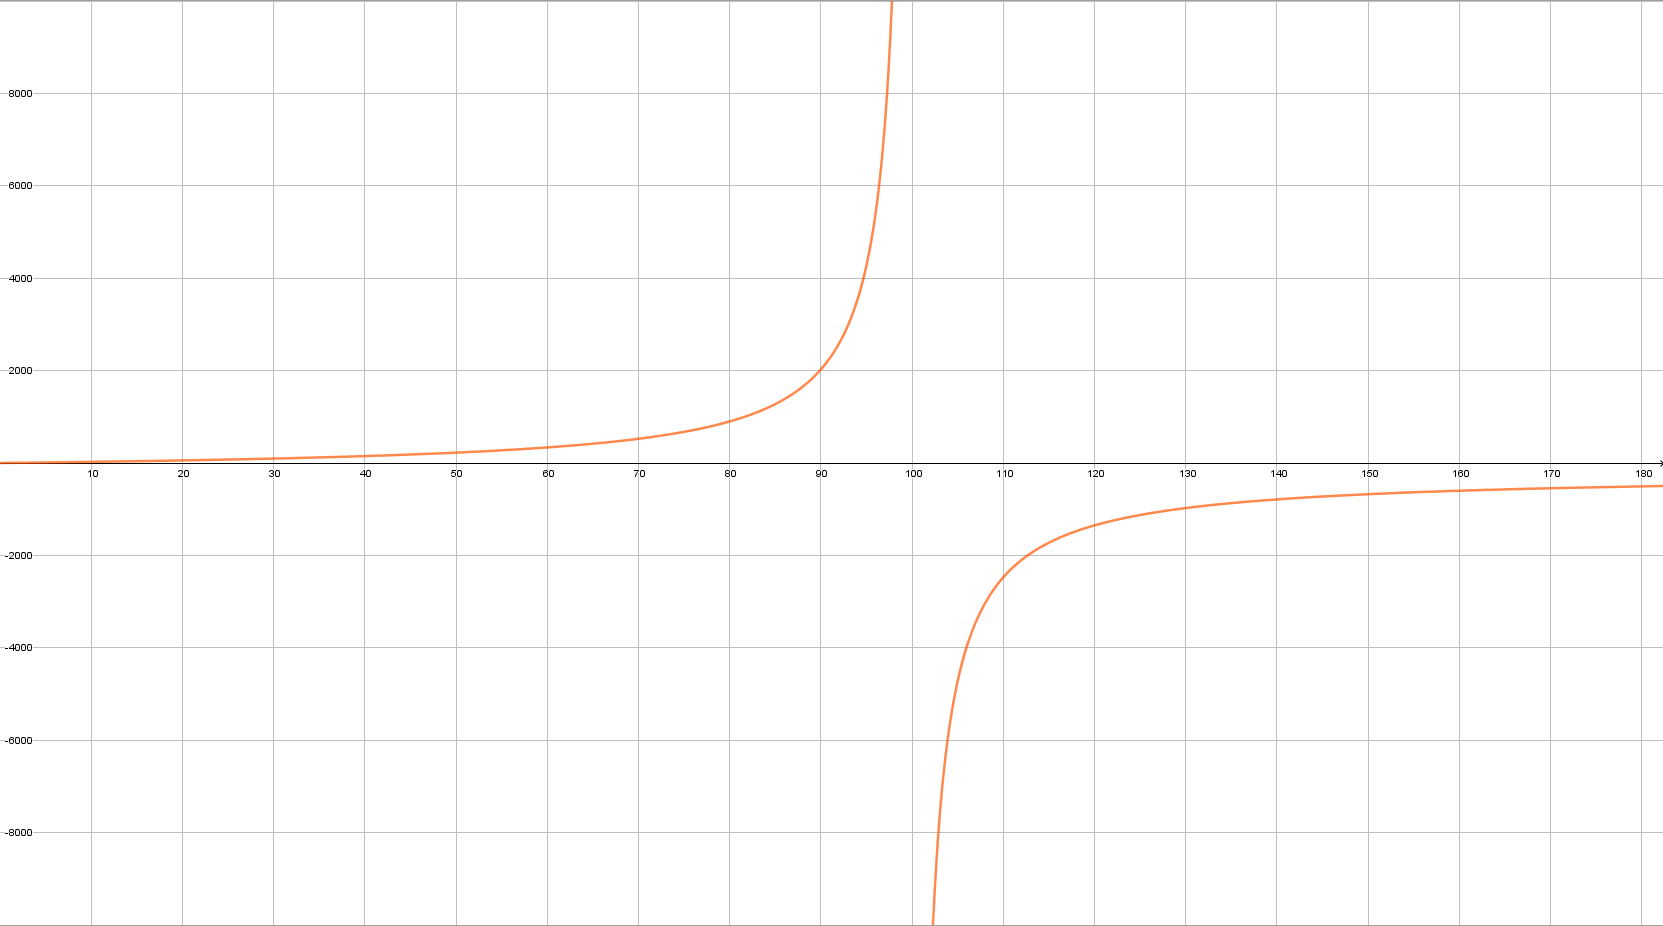
\includegraphics[width=3in]{4142.png}
	
	(b) We need to find $C$ when $p = 10$, when $p = 40$, and when $p = 75$. I used a graphing calculator to do this. \\
	\begin{tabular}{c|ccc}
		$p$ & 10 & 40 & 75 \\ \hline
		$C$ & 25 & 150 & 675
	\end{tabular}

	(c) The graph has a vertical asymptote at $p = 100$, so it is not possible to remove 100\% of the pollutants.
	
	% \vspace{}
	\vfill \newpage
	
	\begin{bex}{4.1.44}
		{
			
		}
	\end{bex} \vspace{-8pt}
	
	% My answer here
	(a) Using GeoGebra: \\
	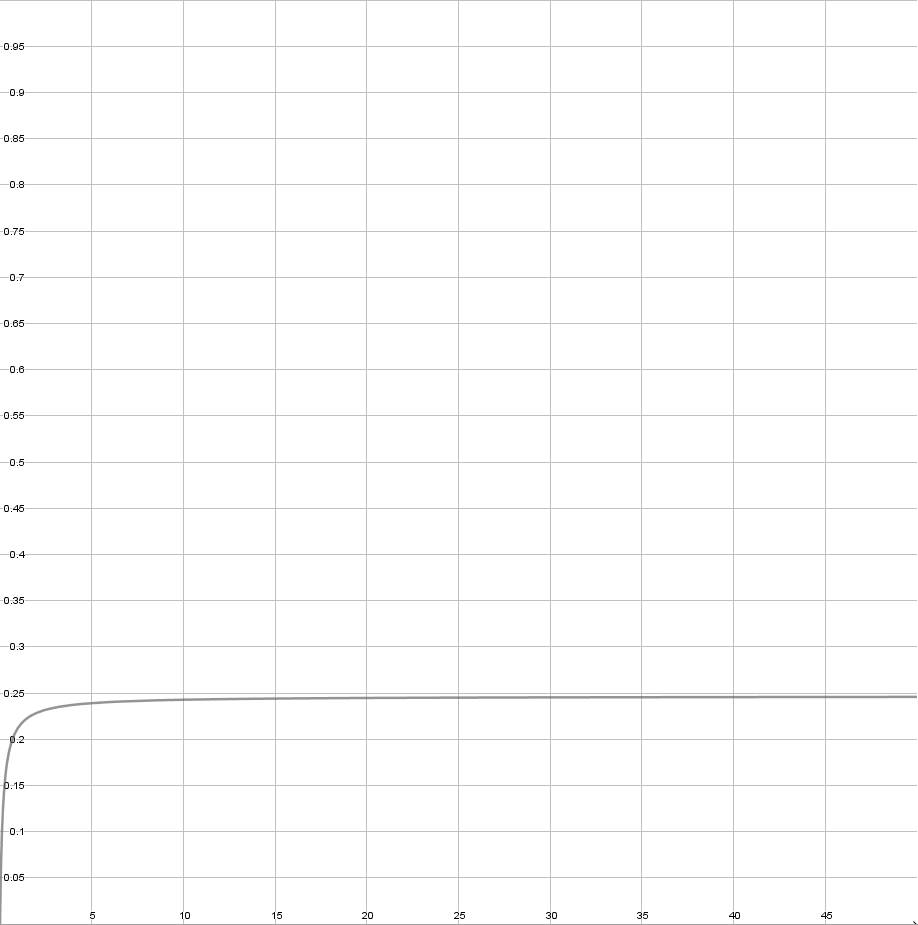
\includegraphics[width=3in]{4144.png}
	
	(b) The word \textit{satiated} means ``full." We are asked to determine how much the moth will eat before it gets full and doesn't eat any more. The graph has a horizontal asymptote at $y = \dfrac{1.568}{6.360} \approx 0.247$, so the moth will be satiated at a level of consumption of about $0.247$ mg.
	
	% \vspace{}
	\vfill % \newpage
	
	
	
\end{document}